\documentclass[10pt,a4paper]{article}

%double si on veut une version prof et une version élève. simple si on veut une seule version.
\newcommand{\buildmode}{double}

\InputIfFileExists{version.tex}{}{}
% Version (définie par le script)
\providecommand{\version}{eleve}

\usepackage{feuilledistanciel}

%%%à modifier à chaque fois

\renewcommand{\niveau}{1G}
\renewcommand{\chapitre}{Révisions}
\renewcommand{\numchap}{0 à 2}
\renewcommand{\theme}{Travail en distanciel}

%%% Arbre pondéré à deux niveaux (pour compléter)
%%% #1, #2 : évènements du 1er niveau ; #3, #4 : évènements du 2nd niveau
\newcommand{\arbrevide}[4]{
\begin{center}
\begin{tikzpicture}[
  grow'=right,
  level distance=3.2cm,
  level 1/.style={sibling distance=2.4cm},
  level 2/.style={sibling distance=1.9cm},
  edge from parent/.style={draw,-latex},
  every node/.style={font=\small}
]
\node {}
  child { node {\(#1\)}
    child { node {\(#3\)} edge from parent node[above] {\(\dots\)} }
    child { node {\(#4\)} edge from parent node[below] {\(\dots\)} }
    edge from parent node[above] {\(\dots\)}
  }
  child { node {\(#2\)}
    child { node {\(#3\)} edge from parent node[above] {\(\dots\)} }
    child { node {\(#4\)} edge from parent node[below] {\(\dots\)} }
    edge from parent node[below] {\(\dots\)}
  };
\end{tikzpicture}
\end{center}
}

\begin{document}

\montitre{Révisions des premiers chapitres}

\textbf{Consignes de travail.} Traiter les sections dans l'ordre. Dans chaque section, commencer par les calculs de début de cours, sans calculatrice, puis lire attentivement le rappel de cours avant de traiter les exercices. Rédiger les réponses sur une copie, en justifiant chaque étape. Chercher d'abord seul, puis lire les indications seulement en cas de blocage. Comparer enfin avec la correction et reprendre ses erreurs d'une autre couleur.

\medskip

\begin{objectifs}
Développer, factoriser une expression et résoudre une équation produit nul.\par\smallskip
Dresser le tableau de signes d'une fonction affine, par le calcul ou graphiquement.\par\smallskip
Dresser le tableau de signes d'un produit de fonctions affines et résoudre une inéquation produit.\par\smallskip
Calculer les termes d'une suite définie explicitement ou par récurrence.\par\smallskip
Étudier le sens de variation d'une suite à l'aide du signe de \(u_{n+1}-u_n\).\par\smallskip
Calculer et interpréter \(P(A\cap B)\) et \(P_A(B)\) à partir d'un tableau croisé.\par\smallskip
Construire et utiliser un arbre pondéré (règle du produit).
\end{objectifs}

\prof{
    Fiche de révision des chapitres 0 (révisions sur les fonctions), 1 (suites, généralités) et 2 (probabilités conditionnelles). Les calculs de début de cours reprennent les automatismes des semaines S1 à S3 de la progression. La formule des probabilités totales n'a pas été vue : aucun calcul de \(P(B)\) par sommation des chemins. Durée indicative : 3 h d'exercices, puis 1 h de feuille blanche.
}

%%%%%%%%%%%%%%%%%%%%%%%%%%%%%%%%%%%%%%%%%%%%%%%%%%%%%%%%%%%%%%%%%%%%%%%%%%%%%
\section{Fonctions affines et produits de fonctions affines}

\begin{exo}[Calculs de début de cours]
Sans calculatrice.
\begin{enumerate}[leftmargin=*]
    \item Développer et réduire :
    \begin{tasks}(2)
        \task \(3(2x-5)\)
        \task \((x+2)(x-3)\)
        \task \((2x-1)(-x+4)\)
        \task \(-(x-1)(x+5)\)
    \end{tasks}
    \item Factoriser :
    \begin{tasks}(3)
        \task \(5x-10\)
        \task \(x^2+3x\)
        \task \((x+1)(2x-3)+(x+1)(x+4)\)
    \end{tasks}
    \item Pour chacune des égalités suivantes, dire s'il s'agit d'une identité (vraie pour toute valeur de \(x\)) ou d'une équation.
    \begin{tasks}(4)
        \task \(2(x+3)=2x+6\)
        \task \(2x+3=7\)
        \task \((x+1)^2=x^2+2x+1\)
        \task \((x+1)^2=x^2+1\)
    \end{tasks}
\end{enumerate}
\end{exo}

\begin{rappelcours}
\textbf{Fonction affine} \(f(x)=ax+b\) : sa courbe est une droite de coefficient directeur \(a\) et d'ordonnée à l'origine \(b\). Si \(a>0\), \(f\) est croissante ; si \(a<0\), \(f\) est décroissante.

\smallskip

\textbf{Signe de \(ax+b\)} (avec \(a\neq 0\)) : \(ax+b\) s'annule en \(x=-\dfrac{b}{a}\).
\begin{itemize}
    \item \textit{Méthode 1 (par le calcul)} : résoudre \(ax+b\geq 0\). Diviser par un nombre négatif change le sens de l'inégalité.
    \item \textit{Méthode 2 (graphique)} : tracer l'allure de la droite à l'aide du signe de \(a\) ; \(ax+b\) est du signe de \(a\) à droite de \(-\dfrac{b}{a}\), et du signe contraire à gauche.
\end{itemize}

\textbf{Signe d'un produit} : on dresse une ligne par facteur, puis on applique la règle des signes sur la dernière ligne. Un produit est nul si et seulement si l'un de ses facteurs est nul.
\end{rappelcours}

\begin{exo}[Guidé]
On considère la fonction \(f\) définie sur \(\mathbb{R}\) par \(f(x)=(3x-2)(-x+4)\). On pose \(u(x)=3x-2\) et \(v(x)=-x+4\).
\begin{enumerate}[leftmargin=*]
    \item Résoudre \(u(x)=0\). Donner le signe du coefficient directeur de \(u\), puis dresser le tableau de signes de \(u\).
    \item Faire de même pour \(v\).
    \item Dresser le tableau de signes de \(f\) : une ligne pour \(u(x)\), une ligne pour \(v(x)\), une ligne pour \(f(x)\).
    \item En déduire l'ensemble des solutions de l'inéquation \(f(x)\geq 0\).
    \item Contrôler la cohérence du tableau en calculant \(f(0)\) et \(f(5)\).
\end{enumerate}

\begin{indication}
Pour le signe de \(ax+b\), faire un schéma rapide de la droite : elle monte si \(a>0\), descend si \(a<0\), et coupe l'axe des abscisses en \(-\dfrac{b}{a}\).
\end{indication}

\checkpoint{\(f(1)=3\), donc \(f(1)\) est positif : le tableau de signes doit indiquer \og \(+\) \fg{} entre les deux valeurs qui annulent \(f\).}
\end{exo}

\begin{exo}
On considère une fonction \(f\) définie sur \([-2,5\ ;\ 3,5]\), dont la représentation graphique est donnée ci-dessous.

\begin{center}
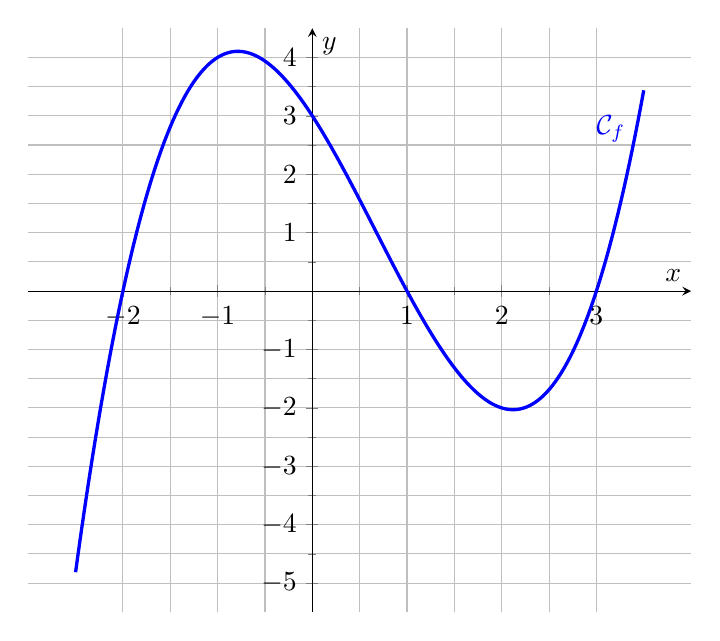
\begin{tikzpicture}
\begin{axis}[
    axis lines=middle,
    xmin=-3, xmax=4,
    ymin=-5.5, ymax=4.5,
    grid=both,
    minor tick num=1,
    xtick={-2,-1,...,3},
    ytick={-5,-4,...,4},
    xlabel={\(x\)},
    ylabel={\(y\)},
    width=10cm,
    height=9cm
]
\addplot[blue, very thick, domain=-2.5:3.5, samples=200] {0.5*(x+2)*(x-1)*(x-3)}
node[pos=0.97, left] {\(\mathcal{C}_f\)};
\end{axis}
\end{tikzpicture}
\end{center}

\begin{enumerate}[leftmargin=*]
    \item Donner l'image de \(0\) et l'image de \(2\) par \(f\).
    \item Donner les antécédents de \(0\) par \(f\).
    \item Dresser le tableau de signes de \(f\) sur \([-2,5\ ;\ 3,5]\).
    \item Résoudre graphiquement l'inéquation \(f(x)\geq 0\).
    \item On admet que \(f(x)=0,5(x+2)(x-1)(x-3)\). Calculer \(f(0)\) et \(f(2)\), et comparer avec la question 1.
\end{enumerate}
\end{exo}

\begin{exo}
Les fonctions suivantes sont définies sur \(\mathbb{R}\). Pour chacune, donner son sens de variation, puis dresser son tableau de signes par les deux méthodes du rappel de cours.
\begin{tasks}(4)
    \task \(f(x)=3x-6\)
    \task \(g(x)=-4x+2\)
    \task \(h(x)=x+5\)
    \task \(k(x)=-x-3\)
\end{tasks}
\end{exo}

\begin{exo}
Pour chacune des fonctions suivantes, dresser le tableau de signes, puis résoudre l'inéquation demandée.
\begin{enumerate}[leftmargin=*]
    \item \(f(x)=(x+2)(2x-5)\) ; résoudre \(f(x)<0\).
    \item \(g(x)=(-3x+1)(x+4)\) ; résoudre \(g(x)\geq 0\).
    \item \(h(x)=x(4-x)\) ; résoudre \(h(x)>0\).
\end{enumerate}
\end{exo}

\begin{exo}[][appro]
On considère la fonction \(f\) définie sur \(\mathbb{R}\) par \(f(x)=2x^2-3x-2\).
\begin{enumerate}[leftmargin=*]
    \item Expliquer pourquoi il n'est pas possible de dresser directement le tableau de signes de \(f\) avec les méthodes de cette section.
    \item Développer \((2x+1)(x-2)\). Que peut-on en déduire ?
    \item Dresser le tableau de signes de \(f\), puis résoudre l'inéquation \(f(x)<0\).
\end{enumerate}
\end{exo}

\prof{
    Exercice 6, question 2 : rédiger avec soin (\og on a montré que \ldots{} ; or \ldots{} ; donc \ldots \fg{}). Ouverture sur le chapitre du second degré.
}

%%%%%%%%%%%%%%%%%%%%%%%%%%%%%%%%%%%%%%%%%%%%%%%%%%%%%%%%%%%%%%%%%%%%%%%%%%%%%
\section{Suites, généralités}

\begin{exo}[Calculs de début de cours]
Sans calculatrice.
\begin{enumerate}[leftmargin=*]
    \item Résoudre les équations produit nul suivantes.
    \begin{tasks}(3)
        \task \((x-3)(2x+5)=0\)
        \task \(x(x+7)=0\)
        \task \((4-x)(3x-1)=0\)
    \end{tasks}
    \item Factoriser, puis résoudre.
    \begin{tasks}(2)
        \task \(x^2-4x=0\)
        \task \(2x^2+6x=0\)
    \end{tasks}
    \item Dans cette question, \(n\) désigne un entier naturel. Donner le signe de chaque expression.
    \begin{tasks}(4)
        \task \(2n+3\)
        \task \(-5\)
        \task \(n^2+1\)
        \task \(-2n-1\)
    \end{tasks}
\end{enumerate}
\end{exo}

\begin{rappelcours}
Une \textbf{suite} \((u_n)\) associe à chaque entier naturel \(n\) un nombre \(u_n\), appelé terme de rang \(n\).
\begin{itemize}
    \item \textbf{Définition explicite} : \(u_n=f(n)\). On peut calculer directement n'importe quel terme, par exemple \(u_{100}\).
    \item \textbf{Définition par récurrence} : on donne le premier terme (par exemple \(u_0\)) et une relation entre \(u_{n+1}\) et \(u_n\). On calcule les termes de proche en proche.
    \item \textbf{Attention :} \(u_{n+1}\) est le terme qui suit \(u_n\) : on l'obtient en remplaçant \(n\) par \(n+1\). En général, \(u_{n+1}\neq u_n+1\).
    \item \textbf{Sens de variation} : on étudie le signe de \(u_{n+1}-u_n\). Si, pour tout \(n\), \(u_{n+1}-u_n\geq 0\), la suite est croissante ; si, pour tout \(n\), \(u_{n+1}-u_n\leq 0\), elle est décroissante.
    \item \textbf{Représentation graphique} : nuage des points de coordonnées \((n\ ;\ u_n)\). Les points sont isolés et ne sont pas reliés.
\end{itemize}
\end{rappelcours}

\begin{exo}[Guidé]
On considère la suite \((u_n)\) définie pour tout entier naturel \(n\) par \(u_n=n^2-4n+3\).
\begin{enumerate}[leftmargin=*]
    \item Calculer \(u_0\), \(u_1\), \(u_2\), \(u_3\), \(u_4\) et \(u_5\).
    \item Représenter le nuage de points correspondant dans le repère ci-dessous.

    \begin{center}
    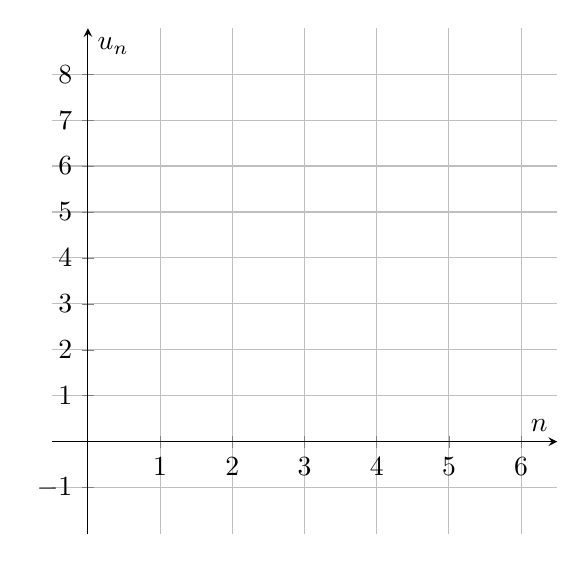
\begin{tikzpicture}
    \begin{axis}[
        axis lines=middle,
        xmin=-0.5, xmax=6.5,
        ymin=-2, ymax=9,
        grid=major,
        xtick={0,1,...,6},
        ytick={-1,0,...,8},
        xlabel={\(n\)},
        ylabel={\(u_n\)},
        width=8cm,
        height=8cm
    ]
    \end{axis}
    \end{tikzpicture}
    \end{center}
    \item Conjecturer le sens de variation de la suite à partir du rang \(2\).
    \item Exprimer \(u_{n+1}\) en fonction de \(n\), puis développer et réduire.
    \item Montrer que, pour tout entier naturel \(n\), \(u_{n+1}-u_n=2n-3\).
    \item Pour quels entiers naturels \(n\) a-t-on \(2n-3\geq 0\) ? Conclure sur le sens de variation de la suite à partir du rang \(2\).
\end{enumerate}

\begin{indication}
Pour obtenir \(u_{n+1}\), remplacer chaque \(n\) par \((n+1)\), avec des parenthèses : \((n+1)^2=n^2+2n+1\).
\end{indication}

\checkpoint{pour \(n=0\), la formule de la question 5 donne \(u_1-u_0=-3\), ce que l'on retrouve avec la question 1.}
\end{exo}

\begin{exo}
Pour chacune des suites suivantes, calculer \(u_1\), \(u_2\) et \(u_4\), puis préciser son mode de définition en justifiant par une phrase.
\begin{enumerate}[leftmargin=*]
    \item \(u_n=3n^2-1\) pour tout entier naturel \(n\).
    \item \(u_0=1\) et, pour tout entier naturel \(n\), \(u_{n+1}=u_n+2n\).
    \item \(u_n=\dfrac{n+1}{n+2}\) pour tout entier naturel \(n\).
    \item \(u_0=-2\) et, pour tout entier naturel \(n\), \(u_{n+1}=-2u_n+1\).
\end{enumerate}
Pour la suite 1, exprimer \(u_{n+1}\) en fonction de \(n\).
\end{exo}

\begin{exo}
Pour chacune des suites suivantes, définies pour tout entier naturel \(n\), calculer \(u_{n+1}-u_n\), puis en déduire le sens de variation de la suite.
\begin{tasks}(3)
    \task \(u_n=5n-2\)
    \task \(u_n=-3n+7\)
    \task \(u_n=n^2+2n\)
    \task \(u_n=\dfrac{1}{n+2}\)
    \task \(u_0=4\) et \(u_{n+1}=u_n-n^2-1\)
\end{tasks}
\end{exo}

\begin{exo}[][appro]
\begin{enumerate}[leftmargin=*]
    \item On donne les premiers termes d'une suite \((u_n)\).

    \begin{center}
    \renewcommand{\arraystretch}{1.5}
    \begin{tabular}{|c|c|c|c|c|c|c|}
        \hline
        \(n\) & \(0\) & \(1\) & \(2\) & \(3\) & \(4\) & \(5\) \\ \hline
        \(u_n\) & \(2\) & \(5\) & \(8\) & \(11\) & \(14\) & \(17\) \\ \hline
    \end{tabular}
    \end{center}
    Proposer une définition explicite et une définition par récurrence cohérentes avec ces valeurs.
    \item Dire si chacune des affirmations suivantes est vraie ou fausse, en justifiant. Utiliser un contre-exemple si nécessaire.
    \begin{enumerate}
        \item Si, pour tout entier naturel \(n\), \(u_{n+1}-u_n=3\), alors la suite \((u_n)\) est croissante.
        \item Si \(u_0<u_1\), alors la suite \((u_n)\) est croissante.
    \end{enumerate}
\end{enumerate}
\end{exo}

\prof{
    Exercice 11 : rappeler que quelques termes ne suffisent pas à prouver une formule ; ici on demande une définition \og cohérente \fg{} avec les valeurs, pas \og la \fg{} définition.
}

%%%%%%%%%%%%%%%%%%%%%%%%%%%%%%%%%%%%%%%%%%%%%%%%%%%%%%%%%%%%%%%%%%%%%%%%%%%%%
\section{Probabilités conditionnelles}

\begin{exo}[Calculs de début de cours]
Sans calculatrice.
\begin{enumerate}[leftmargin=*]
    \item Compléter le tableau suivant.

    \begin{center}
    \renewcommand{\arraystretch}{1.8}
    \begin{tabular}{|c|c|c|c|c|c|}
        \hline
        Fraction & \(\dfrac{3}{4}\) & \(\dfrac{2}{5}\) & \(\dots\) & \(\dots\) & \(\dfrac{7}{20}\) \\ \hline
        Décimal & \(\dots\) & \(\dots\) & \(0,15\) & \(\dots\) & \(\dots\) \\ \hline
        Pourcentage & \(\dots\) & \(\dots\) & \(\dots\) & \(12,5\,\%\) & \(\dots\) \\ \hline
    \end{tabular}
    \end{center}
    \item On considère l'univers \(\Omega=\{1;2;3;4;5;6;7;8;9;10\}\) et les évènements \(A=\{2;4;6;8;10\}\) et \(B=\{1;2;3;4\}\).
    \begin{enumerate}
        \item Écrire les ensembles \(A\cap B\), \(A\cup B\) et \(\overline{A}\).
        \item Donner \(\mathrm{Card}(A\cap B)\).
        \item Vrai ou faux : \(4\in A\cap B\) ; \(A\subset B\) ; \(\{2;4\}\subset B\).
    \end{enumerate}
\end{enumerate}
\end{exo}

\begin{rappelcours}
\(P(A\cap B)\) est la probabilité que \(A\) \textbf{et} \(B\) se réalisent.

\smallskip

Si \(P(A)\neq 0\), la \textbf{probabilité de \(B\) sachant \(A\)} est \(P_A(B)=\dfrac{P(A\cap B)}{P(A)}\). Dans un tableau d'effectifs, en situation d'équiprobabilité, on se restreint à la ligne ou à la colonne de \(A\) : \(P_A(B)=\dfrac{\mathrm{Card}(A\cap B)}{\mathrm{Card}(A)}\). En général, \(P_A(B)\neq P_B(A)\).

\smallskip

\textbf{Arbre pondéré} : le premier niveau porte \(P(A)\) et \(P(\overline{A})\) ; le second niveau porte des probabilités conditionnelles, comme \(P_A(B)\). La somme des probabilités des branches issues d'un même nœud vaut \(1\).

\smallskip

\textbf{Règle du produit} : la probabilité d'un chemin est le produit des probabilités portées par ses branches : \(P(A\cap B)=P(A)\times P_A(B)\).
\end{rappelcours}

\begin{exo}[Guidé]
Une médiathèque de Saint-Denis a interrogé \(250\) usagers. Le tableau donne la répartition selon l'âge et l'emprunt de bandes dessinées (BD).

\begin{center}
\renewcommand{\arraystretch}{1.5}
\begin{tabular}{|l|c|c|c|}
    \hline
    & \textbf{Mineurs} & \textbf{Majeurs} & \textbf{Total} \\ \hline
    \textbf{Empruntent des BD} & \(60\) & \(40\) & \(100\) \\ \hline
    \textbf{N'empruntent pas de BD} & \(30\) & \(120\) & \(150\) \\ \hline
    \textbf{Total} & \(90\) & \(160\) & \(250\) \\ \hline
\end{tabular}
\end{center}

On choisit un usager au hasard. On note \(M\) l'évènement \og l'usager est mineur \fg{} et \(B\) l'évènement \og l'usager emprunte des BD \fg{}.
\begin{enumerate}[leftmargin=*]
    \item Calculer \(P(M)\).
    \item Traduire l'évènement \(M\cap B\) par une phrase, puis calculer \(P(M\cap B)\).
    \item Calculer \(P_M(B)\) en se restreignant à la colonne des mineurs. Traduire ce résultat par une phrase.
    \item Calculer \(P_B(M)\). Comparer avec la question 3.
    \item Vérifier que \(P_M(B)=\dfrac{P(M\cap B)}{P(M)}\).
\end{enumerate}

\begin{indication}
\og Sachant que l'usager est mineur \fg{} : l'univers se réduit aux \(90\) mineurs. \og Sachant que l'usager emprunte des BD \fg{} : il se réduit aux \(100\) emprunteurs de BD.
\end{indication}

\checkpoint{\(P_M(B)\) et \(P_B(M)\) sont deux nombres différents, tous deux supérieurs à \(0,5\).}
\end{exo}

\begin{exo}
Une plateforme de streaming propose deux offres. \(40\,\%\) des abonnés ont l'offre Premium. Parmi les abonnés Premium, \(75\,\%\) regardent des séries chaque semaine. Parmi les autres abonnés, \(50\,\%\) regardent des séries chaque semaine.

On choisit un abonné au hasard. On note \(P\) l'évènement \og l'abonné a l'offre Premium \fg{} et \(S\) l'évènement \og l'abonné regarde des séries chaque semaine \fg{}.
\begin{enumerate}[leftmargin=*]
    \item Recopier et compléter l'arbre pondéré ci-dessous.
    \arbrevide{P}{\overline{P}}{S}{\overline{S}}
    \item Écrire la probabilité \(0,75\) de l'énoncé avec la notation \(P_{\dots}(\dots)\).
    \item Calculer \(P(P\cap S)\), puis \(P(P\cap\overline{S})\). Traduire ce dernier résultat par une phrase.
    \item Calculer la probabilité que l'abonné choisi n'ait pas l'offre Premium et ne regarde pas de séries chaque semaine.
    \item Parmi les probabilités \(P(P\cap S)\), \(P_P(S)\) et \(P_S(P)\), indiquer celle qui peut être lue directement sur l'arbre, celle qui se calcule avec la règle du produit, et celle qui ne peut être obtenue ni par l'une ni par l'autre.
\end{enumerate}
\end{exo}

\begin{exo}
Une entreprise a interrogé ses \(200\) salariés sur la durée de leur trajet et sur le télétravail.

\begin{center}
\renewcommand{\arraystretch}{1.5}
\begin{tabular}{|l|c|c|c|}
    \hline
    & \textbf{Télétravail} & \textbf{Pas de télétravail} & \textbf{Total} \\ \hline
    \textbf{Trajet de plus d'une heure} & \(45\) & \(15\) & \(60\) \\ \hline
    \textbf{Trajet d'une heure ou moins} & \(35\) & \(105\) & \(140\) \\ \hline
    \textbf{Total} & \(80\) & \(120\) & \(200\) \\ \hline
\end{tabular}
\end{center}

On choisit un salarié au hasard. On note \(L\) l'évènement \og le trajet dure plus d'une heure \fg{} et \(T\) l'évènement \og le salarié est en télétravail \fg{}.
\begin{enumerate}[leftmargin=*]
    \item À l'aide du tableau, calculer les probabilités nécessaires, puis recopier et compléter l'arbre pondéré ci-dessous.
    \arbrevide{L}{\overline{L}}{T}{\overline{T}}
    \item Calculer \(P(L\cap T)\) à l'aide de l'arbre, puis à l'aide du tableau. Vérifier que les deux résultats sont égaux.
    \item Calculer \(P_T(L)\). Interpréter ce résultat dans le contexte.
\end{enumerate}
\end{exo}

\begin{exo}[][appro]
\begin{enumerate}[leftmargin=*]
    \item Soit \(A\) et \(B\) deux évènements tels que \(P(A)=x\), \(P_A(B)=0,6\) et \(P_{\overline{A}}(B)=0,2\), où \(x\) est un réel de \(]0\ ;\ 1[\). On sait de plus que \(P(A\cap B)=0,24\).
    \begin{enumerate}
        \item Construire l'arbre pondéré correspondant, en exprimant les probabilités du premier niveau en fonction de \(x\).
        \item Écrire une équation vérifiée par \(x\), puis la résoudre.
        \item En déduire \(P(\overline{A}\cap B)\).
    \end{enumerate}
    \item Soit \(C\) et \(D\) deux évènements tels que \(P(C)=0,3\), \(P_C(D)=y\) et \(P(C\cap\overline{D})=0,12\). Déterminer \(y\).
\end{enumerate}
\end{exo}

\prof{
    Exercice 16 : lien avec les calculs de début de cours (résolution d'équations). Pour la question 2, exprimer d'abord \(P_C(\overline{D})\) en fonction de \(y\).
}

%%%%%%%%%%%%%%%%%%%%%%%%%%%%%%%%%%%%%%%%%%%%%%%%%%%%%%%%%%%%%%%%%%%%%%%%%%%%%
\section{Problèmes}

Les problèmes suivants mélangent les notions des trois sections précédentes.

\begin{exo}[Abonnés d'une plateforme]
Au 1\ier{} janvier 2026, une plateforme compte \(2\,000\) abonnés. Chaque mois, \(10\,\%\) des abonnés se désabonnent et \(300\) nouvelles personnes s'abonnent. On note \(a_n\) le nombre d'abonnés \(n\) mois après le 1\ier{} janvier 2026 ; ainsi \(a_0=2\,000\).
\begin{enumerate}[leftmargin=*]
    \item Calculer \(a_1\) et \(a_2\).
    \item Justifier que, pour tout entier naturel \(n\), \(a_{n+1}=0,9\,a_n+300\). Préciser le mode de définition de la suite \((a_n)\).
    \item Calculer \(a_3\) et \(a_4\) (arrondir à l'unité), puis conjecturer le sens de variation de la suite \((a_n)\).
    \item On admet que, pour tout entier naturel \(n\), \(a_n=3\,000-1\,000\times 0,9^n\).
    \begin{enumerate}
        \item Vérifier cette formule pour \(n=0\) et \(n=1\).
        \item Montrer que, pour tout entier naturel \(n\), \(a_{n+1}-a_n=100\times 0,9^n\).
        \item En déduire le sens de variation de la suite \((a_n)\).
    \end{enumerate}
\end{enumerate}

\begin{indication}
Pour la question 4b, remarquer que \(0,9^{n+1}=0,9\times 0,9^n\), puis factoriser par \(0,9^n\).
\end{indication}
\end{exo}

\begin{exo}[Une petite entreprise]
Une entreprise fabrique entre \(0\) et \(1\,200\) objets par semaine. On note \(x\) le nombre d'objets fabriqués, en centaines, avec \(x\in[0\ ;\ 12]\). Le bénéfice hebdomadaire, en milliers d'euros, est modélisé par
\[ B(x)=(x-2)(-3x+30). \]
\begin{enumerate}[leftmargin=*]
    \item Calculer \(B(0)\) et interpréter le résultat.
    \item Dresser le tableau de signes de \(B\) sur \([0\ ;\ 12]\).
    \item En déduire les quantités d'objets pour lesquelles l'entreprise réalise un bénéfice.
    \item Les objets sont fabriqués sur deux chaînes : \(70\,\%\) par la chaîne \(A\), les autres par la chaîne \(\overline{A}\). Parmi les objets de la chaîne \(A\), \(2\,\%\) sont défectueux ; parmi ceux de la chaîne \(\overline{A}\), \(5\,\%\) sont défectueux. On choisit un objet au hasard et on note \(D\) l'évènement \og l'objet est défectueux \fg{}.
    \begin{enumerate}
        \item Construire l'arbre pondéré de la situation.
        \item Calculer \(P(A\cap D)\) et \(P(\overline{A}\cap D)\).
        \item Le responsable affirme : \og La chaîne \(A\) fabrique plus d'objets, donc c'est elle qui fournit le plus d'objets défectueux. \fg{} Que penser de cette affirmation ?
    \end{enumerate}
\end{enumerate}
\end{exo}

\prof{
    Exercice 18 : on ne demande pas \(P(D)\), qui relève de la formule des probabilités totales.
}

%%%%%%%%%%%%%%%%%%%%%%%%%%%%%%%%%%%%%%%%%%%%%%%%%%%%%%%%%%%%%%%%%%%%%%%%%%%%%
\section{Bilan}

Réaliser une très longue feuille blanche (1 h, soit \(3\times 20\) minutes) sur ce qui a été fait dans cette feuille. On rappelle que les objectifs de cette feuille étaient les suivants :

\medskip

Développer, factoriser une expression et résoudre une équation produit nul.\par\smallskip
Dresser le tableau de signes d'une fonction affine, par le calcul ou graphiquement.\par\smallskip
Dresser le tableau de signes d'un produit de fonctions affines et résoudre une inéquation produit.\par\smallskip
Calculer les termes d'une suite définie explicitement ou par récurrence.\par\smallskip
Étudier le sens de variation d'une suite à l'aide du signe de \(u_{n+1}-u_n\).\par\smallskip
Calculer et interpréter \(P(A\cap B)\) et \(P_A(B)\) à partir d'un tableau croisé.\par\smallskip
Construire et utiliser un arbre pondéré (règle du produit).

\prof{
    Feuille blanche : rappeler qu'elle est personnelle, sans cours ni fiche. Possibilité de la faire en trois temps de 20 minutes, en relisant la fiche entre deux temps.
}

\end{document}
